\begin{frame}{What is a game?}
	\begin{quotation}
		\centering
		Game theory is the mathematical study of {\color{green!60!black}interaction}\\ among independent, self-interested {\color{blue}agents}.\\
		{\color{colornote}-- Essentials of Game Theory \cite{leyton2008essentials}}
	\end{quotation}

	\vfill
	\textbf{Examples}: economic games, proof theory, machine learning, control theory, etc.

	\vfill
	A game factors in two parts:
	\begin{enumerate}
		\item An \textcolor{colorarena}{\textbf{arena}}, which models the {interaction patterns} in the game
		\item \textcolor{blue}{\textbf{Players}}, which intervene in the arena by making \textbf{decisions} at different points
	\end{enumerate}

	\vfill
	\begin{center}
		\includegraphics[width=.7\textwidth]{figures/board-games.png}
	\end{center}
	\vspace{-3ex}
\end{frame}

\begin{frame}{What is a game?}
	An \textcolor{colorarena}{arena} is an open system with three boundaries:

	\begin{center}
		\includegraphics[clip, page=2, trim=0cm 3cm 3cm 2cm, width=.8\textwidth]{figures/drawings.pdf}
	\end{center}

	This is a parametrised lens $\textcolor{colorarena}{\A : (X,S) \nlongto{\textcolor{coloragents}{(\Omega, \Comega)}} (Y,R)}$ specified by two maps
	\begin{eqalign*}
		\textcolor{colorarena}{\play} &: \textcolor{coloragents}{\Omega} \textcolor{colorarena}{\times X \to Y},\\
		\textcolor{colorarena}{\coplay} &: \textcolor{coloragents}{\Omega} \textcolor{colorarena}{\times X \times R \to \textcolor{coloragents}{\Comega} \times S}
	\end{eqalign*}
\end{frame}

\begin{frame}{What is a game?}
	It can be closed by specifying an \textbf{initial state} and a \textbf{utility function}:

	\begin{center}
		\fbox{\includegraphics[clip, page=4, trim=4.5cm 2cm 3cm 6cm, width=.9\textwidth]{figures/drawings.pdf}}
	\end{center}
\end{frame}

\begin{frame}{What is a game?}
	At the end of the day, the \textcolor{colorarena}{arena} amounts to an evaluation of strategies with rewards:

	\vspace{5ex}
	\begin{center}
		\fbox{\includegraphics[clip, page=5, trim=3cm 7cm .5cm 5cm, width=.9\textwidth]{figures/drawings.pdf}}
	\end{center}
\end{frame}

\begin{frame}{What is a game?}
	\textcolor{coloragents}{Agents} can then choose which strategies to play using a \textcolor{coloragents}{\textbf{selection function}}:


	\begin{center}
		\includegraphics[clip, page=6, trim=0cm 3cm 3cm 2cm, width=.7\textwidth]{figures/drawings.pdf}
	\end{center}

	\textcolor{colornote}{Typically, $\Omega$ is finite, $\Comega = \R$ and $\varepsilon$ is $\argmax$.}
\end{frame}

\begin{frame}{Interlude: selection functions}
	Let $\S(X,S) := (X \to S) \to \pow{X}$. This is a functor on lenses:
	\begin{eqalign*}
		\S(\alpha) : \S(X,S) &\longto \S(Y,R)\\
		\varepsilon &\longmapsto \lambda k \,.\, \{x \cmp \alpha \suchthat x \in \varepsilon(\alpha \cmp k)\}
	\end{eqalign*}
	where $\alpha : (X, S) \to (Y,R)$ and we implicitly used $\Lens((1,1),(Y,R)) \iso Y \to R$ and $\Lens((X,S),(1,1)) \iso X$:

	(drawing)

	This functor is lax monoidal (\textbf{Nash product}):
	\begin{eqalign*}
		- \boxtimes - : \S(X,S) \times \S(Y,R) &\longto \S(X \times Y, S \times R)\\
		(\varepsilon, \eta) &\longmapsto \lambda k \,.\, \{ (x,y) \suchthat x \in \varepsilon(k_1(x,y))\ \text{and}\ y \in \eta(k_2(x,y))\}
	\end{eqalign*}
	(drawing)

	\textcolor{colornote}{This yields a moncat $\Lens_\S = \underset{mon}\int \S$.}
\end{frame}

\begin{frame}{The definition}
	\begin{definition}
		An \textbf{open game with agency} $\G$ is a pair
		\begin{equation*}
			\colar{\A : (X,S) \nlongto{\colag{(\Omega, \Comega)}} (Y,R)}, \quad \colag{\varepsilon  : \S(\Omega, \Comega)}
		\end{equation*}
		\textcolor{colornote}{More succintly: a $\Lens_\S$-parametrised lens}.
	\end{definition}

	\vfill
	Agency $\neq$ players: players arise from the presentation; if $\Omega = \prod_{p \in P} \Omega_p$, $\Comega = \prod_{p \in P} \Comega_p$ and $\varepsilon = \Boxtimes_{p \in P} \varepsilon_p$ we speak of \textbf{open game with} (set of) \textbf{players $P$}.

	\vfill
	Equilibria for $\G = (\A, \varepsilon)$ are given by:
	\begin{equation*}
		\eq_\G(x, k) = \colag{\varepsilon(}\colar{x \cmp \A \cmp k}\colag{)}.
	\end{equation*}
	%where $(-)^\top : \Lens_{(\Omega, \Comega)}((1,1),(1,1))\ \iso\ \Omega \to \Comega$.
\end{frame}

% Let's focus on arenas, aka parametrised lenses, for a while...
\begin{frame}{Composing arenas}
	\textcolor{colorarena}{Arenas} are the compositional heart of open games with agency:


\end{frame}

\begin{frame}{Composing arenas}

	\textbf{Notice}: as of now, these operators can't be extended to selection functions in a canonical way!
\end{frame}

\begin{frame}{Reparametrisation}
	Most importantly arenas form a (locally fibred) bicategory: one can \textbf{reparametrise} along a lens $\colag{\alpha : (\Omega', \Comega') \to (\Omega, \Comega)}$.

	\vfill
	This is crucial for introducing agency!

	%\vfill
	%\textcolor{colornote}{If we work in $\Para_{\times_\S}(\Lens_\S)$, we see that `$(1,1,\top)$ coclassifies equilibria', i.e. $(1,1,\top) \twoto \G \iso \eq_\G$.}
\end{frame}

\begin{frame}{Regrouping}
	As an example, if $\A$ has set of players $P$ and $r : P \to Q$ is a function, we can turn $\A$ into an arena with players $Q$ by reparametrising along
	\begin{equation*}
		\regroup_r : (\prod_{q \in Q} (r^* \Omega)_q, \prod_{q \in Q} (r^* \Comega)_q) \longto (\prod_{p \in P} \Omega_p, \prod_{p \in P} \Comega_p)
	\end{equation*}
	which only 'regroups' the factors according to $r$.
	\begin{example}
		If $\A_1$ and $\A_2$ have the same players $P$, $\A_1 \cmp \A_2$ has players $P+P$. So we regroup along $P+P \to P$ to get again an arena with players $P$.
	\end{example}
\end{frame}

\begin{frame}{Tying}
	The second most important application for reparametrisations is tying strategies at different point of the game. This is done by reparametrising along $(\Delta, \mathsf{combine})$ (where $\mathsf{combine} = +, \pi_2, \max, \ldots$).

	\vfill
	\textbf{Notice}: $(\Delta, \mathsf{combine})^*(\A_1 \cmp \A_2)$ lies outside the image of $-\cmp-$, hence introduces 'non-compositional' effects. Indeed: \textcolor{coloragents}{agency} is non-local.
	%\textcolor{colornote}{We'll use this soon to treat imperfect information. Also useful for Markov games.}
\end{frame}
